%%%%%%%%%%%%%%%%%%%%%%%%%%%%%%%%%%%%%%%%%%%%%%%%%%%%%%%%%%%%%%%%%%%%%%%%%%%%%%%%
%% Plantilla de memoria en LaTeX para la ETSIT - Universidad Rey Juan Carlos
%%
%% Por Gregorio Robles <grex arroba gsyc.urjc.es>
%%     Grupo de Sistemas y Comunicaciones
%%     Escuela Técnica Superior de Ingenieros de Telecomunicación
%%     Universidad Rey Juan Carlos
%% (muchas ideas tomadas de Internet, colegas del GSyC, antiguos alumnos...
%%  etc. Muchas gracias a todos)
%%
%% La última versión de esta plantilla está siempre disponible en:
%%     https://github.com/gregoriorobles/plantilla-memoria
%%
%% Para obtener PDF, ejecuta en la shell:
%%   make
%% (las imágenes deben ir en PNG o JPG)

%%%%%%%%%%%%%%%%%%%%%%%%%%%%%%%%%%%%%%%%%%%%%%%%%%%%%%%%%%%%%%%%%%%%%%%%%%%%%%%%

\documentclass[a4paper, 12pt]{book}
%\usepackage[T1]{fontenc}

\usepackage[a4paper, left=2.5cm, right=2.5cm, top=3cm, bottom=3cm]{geometry}
\usepackage{times}
\usepackage[latin1]{inputenc}
\usepackage[spanish]{babel} % Comenta esta línea si tu memoria es en inglés
\usepackage{url}
%\usepackage[dvipdfm]{graphicx}
\usepackage{graphicx}
\usepackage{float}  %% H para posicionar figuras
\usepackage[nottoc, notlot, notlof, notindex]{tocbibind} %% Opciones de índice
\usepackage{latexsym}  %% Logo LaTeX

\title{Memoria del Proyecto}
\author{Nombre del autor}

\renewcommand{\baselinestretch}{1.5}  %% Interlineado

\begin{document}

\renewcommand{\refname}{Bibliografía}  %% Renombrando
\renewcommand{\appendixname}{Apéndice}

%%%%%%%%%%%%%%%%%%%%%%%%%%%%%%%%%%%%%%%%%%%%%%%%%%%%%%%%%%%%%%%%%%%%%%%%%%%%%%%%
% PORTADA

\begin{titlepage}
\begin{center}
\begin{tabular}[c]{c c}
%\includegraphics[bb=0 0 194 352, scale=0.25]{logo} &
\includegraphics[scale=0.25]{img/logo_vect.png} &
\begin{tabular}[b]{l}
\Huge
\textsf{UNIVERSIDAD} \\
\Huge
\textsf{REY JUAN CARLOS} \\
\end{tabular}
\\
\end{tabular}

\vspace{3cm}

\Large
GRADO EN TECNOLOGÍAS DE LA TELECOMUNICACIÓN

\vspace{0.4cm}

\large
Curso Académico 2019/2020

\vspace{0.8cm}

Trabajo Fin de Grado

\vspace{2.5cm}

\LARGE
APLICACIÓN WEB DE COMERCIO ELECTRÓNICO PARA UNA TIENDA DE ELECTRODOMÉSTICOS (NEVADO)

\vspace{4cm}

\large
Autor : Sandra Álvarez Gancedo \\
Tutor : Dr. Gregorio Robles
\end{center}
\end{titlepage}

\newpage
\mbox{}
\thispagestyle{empty} % para que no se numere esta pagina


%%%%%%%%%%%%%%%%%%%%%%%%%%%%%%%%%%%%%%%%%%%%%%%%%%%%%%%%%%%%%%%%%%%%%%%%%%%%%%%%
%%%% Para firmar
\clearpage
\pagenumbering{gobble}
\chapter*{}

\vspace{-4cm}
\begin{center}
\LARGE
\textbf{Trabajo Fin de Grado}

\vspace{1cm}
\large
Aplicación web de comercio electrónico para una tienda de electrodomésticos (Nevado)

\vspace{1cm}
\large
\textbf{Autor :} Sandra Álvarez Gancedo\\
\textbf{Tutor :} Dr. Gregorio Robles Martínez

\end{center}

\vspace{1cm}
La defensa del presente Proyecto Fin de Carrera se realizó el día \qquad$\;\,$ de \qquad\qquad\qquad\qquad \newline de 2020, siendo calificada por el siguiente tribunal:


\vspace{0.5cm}
\textbf{Presidente:}

\vspace{1.2cm}
\textbf{Secretario:}

\vspace{1.2cm}
\textbf{Vocal:}


\vspace{1.2cm}
y habiendo obtenido la siguiente calificación:

\vspace{1cm}
\textbf{Calificación:}


\vspace{1cm}
\begin{flushright}
Fuenlabrada, a \qquad$\;\,$ de \qquad\qquad\qquad\qquad de 2020
\end{flushright}

%%%%%%%%%%%%%%%%%%%%%%%%%%%%%%%%%%%%%%%%%%%%%%%%%%%%%%%%%%%%%%%%%%%%%%%%%%%%%%%%
%%%% Dedicatoria

\chapter*{}
\pagenumbering{Roman} % para comenzar la numeracion de paginas en numeros romanos
\begin{flushright}
\textit{Un esfuerzo total \\
es una victoria completa \\
Mahatma Gandhi} 
\end{flushright}

%%%%%%%%%%%%%%%%%%%%%%%%%%%%%%%%%%%%%%%%%%%%%%%%%%%%%%%%%%%%%%%%%%%%%%%%%%%%%%%%
%%%% Agradecimientos

\chapter*{Agradecimientos}
%\addcontentsline{toc}{chapter}{Agradecimientos} % si queremos que aparezca en el índice
\markboth{AGRADECIMIENTOS}{AGRADECIMIENTOS} % encabezado 

En primer lugar quiero agradecer a mis padres, pues sin ellos y sin su esfuerzo no hubiese sido capaz de cerrar este ciclo. Muchas han sido las noches que habéis estado a mi lado, aguantando mis desvelos, mis nervios y mis miedos. Habéis sido el consuelo y el apoyo que necesitaba en mis momentos más duros, en los que únicamente un simple gesto vuestro hacía levantarme. Sois y sereís mi mejor ejemplo a seguir. 

La vida me ha regalado unos segundos padres, mis tios, los cuales me quieren y me protegen como a una hija. Me habéis acompañado en los momentos más felices, pero también en los más difíciles, incluso cuando a mis padres les faltaban fuerzas para seguir adelante. Simplemente deciros, gracias.

Mi primo, más que un hermano. Cuantos momentos vividos, siempre liándola, en las buenas y las no tan buenas, pero siempre juntos. Nos separamos en esta etapa universitaria, pero nuestras carreras eran tan iguales que no nos ha impedido seguir ayudándonos. 

Quiero agradecer a mis abuelos, a mi abuelo por enseñarme lo que es la vida. Por enseñarme que de todo lo malo también hay que saber sacar el lado positivo. A mi abuela, porque sé que desde algún rinconcito del cielo ha visto como lograba alcanzar todos mis sueños y mis metas. Pero sobre todo sé, que desde ahí arriba, me ha ayudado a luchar y a salir hacia delante ante el mayor reto de mi vida. Sé que estarías orgullosa de mí. 

La universidad me ha aportado muchas cosas buenas, pero gracias a ella, conocí a quien es hoy uno de mis pilares, Alejandro. Se ha convertido en mi mejor amigo, mi confidente, mi otra mitad. Gracias por todo lo que has hecho y haces por mí. Me has ayudado en la universidad, pues sin ti, no sé si hubiese sido capaz de aprobar aquella asignatura que me traía por el camino de la amargura. Pero, sobre todo, me has ayudado en la vida, te quedaste a mi lado en el peor momento, cuando a todos nos invadia la incertidumbre, cuando ninguno sabia que iba a pasar, ahí estuviste conmigo. Me has dado fuerzas cuando mas flaqueaba, me has sacado una sonrisa cuando más lo necesitaba, y me has dado entereza para asumir y afrontar lo que me estaba ocurriendo. Ha habido muchos momentos malos durante estos 5 años, pero juntos los hemos superado y así seguiremos haciéndolo. 

Agradecer a mis compañeros y amigos de universidad por todos los apuntes y conocimientos intercambiados.

A mis profesores, en especial a Antonio Marqués y Carlos Figueras, pues me ayudaron, me apoyaron y me dieron facilidades para poder sacar adelante la asignatura PDAC, a pesar de mis condiciones. Recuerdo, con cariño, el email de Antonio para comunicarme que había conseguido aprobar la asignatura y felicitarme por ello, pues sabía del esfuerzo realizado. 

Quiero hacer mención especial a mi tutor de proyecto, Gregorio Robles, por darme ánimos para llegar donde estoy hoy, terminando el trabajo fin de grado. Pero, sobre todo, gracias por ser paciente, por entender y comprender mi situación. 

Y, por último, no me puedo olvidar de todos los médicos y enfermeras que me han atendido durante estos cinco años, puesto que, sin su esfuerzo, su investigación y su predisposición, no hubiese podido terminar esta etapa. 

Agradecer a la vida, porque a pesar de todo he tenido suerte. Suerte por tener a la gente que tengo a mi lado, por haber podido estudiar, pero, sobre todo, suerte porque no todos pueden decir que han superado una enfermedad, como es un linfoma. Y, por qué no, gracias a ti, linfoma, porque me has enseñado a disfrutar y vivir la vida al máximo y a dar importancia a las cosas que realmente las tienen.

%%%%%%%%%%%%%%%%%%%%%%%%%%%%%%%%%%%%%%%%%%%%%%%%%%%%%%%%%%%%%%%%%%%%%%%%%%%%%%%%
%%%% Resumen

\chapter*{Resumen}
%\addcontentsline{toc}{chapter}{Resumen} % si queremos que aparezca en el índice
\markboth{RESUMEN}{RESUMEN} % encabezado

El proyecto tiene como objetivo principal desarrollar una aplicación web de comercio electrónico para la venta de electrodomésticos.

Gracias a aplicaciones como la que se desarrollada en este trabajo, pequeños comercios pueden ampliar su mercado y llegar a más gente, pues simplemente accediendo a la web se puede ver la variedad de productos que hay en el catálago, conocer su precio y realizar la compra de manera sencilla y, sin tener la necesidad de ir a la tienda física. 

Destacar que además de la venta de electrodomésticos, la aplicación permite al administrador, dueño del comercio, gestionar los clientes, los productos, las ofertas, los pedidos y las facturas. Pensando en está gestión, se implementa un sistema de importación y exportación de ficheros excel que permite al administrador cargar por ejemplo, productos de manera masiva sin tener que ir uno a uno, agilizando el trabajo del  administrador. 

La aplicación está diseñada para que cualquier usuario pueda navegar en ella, sin ningún tipo de dificultad. Para ello, se ha tenido en cuenta los criterios de accesibilidad y se han adaptado las distintas vistas a las resoluciones de pantalla más comunes, de tal forma que se pueda manejar tanto en un móvil como en un ordenador, sin que se produzca ningún cambio de usabilidad. Esto ha propiciado que para el desarrollo de la aplicación se  hayan elegido las siguientes tecnologías: HTML5, CSS3, Bootstrap, Angular 7 y TypeScript (para la parte del cliente) y NodeJS, MongoDB y JavaScript (para la parte del servidor).

%%%%%%%%%%%%%%%%%%%%%%%%%%%%%%%%%%%%%%%%%%%%%%%%%%%%%%%%%%%%%%%%%%%%%%%%%%%%%%%%
%%%% Resumen en inglés

\chapter*{Summary}
%\addcontentsline{toc}{chapter}{Summary} % si queremos que aparezca en el índice
\markboth{SUMMARY}{SUMMARY} % encabezado

The main objective of the project is to develop an e-commerce web application for the sale of household appliances.

Thanks to applications like the one developed in this work, small shops can expand their market and reach more people, because simply by accessing the web you can see the variety of products in the catalogue, know their price and make the purchase in a simple way and without having to go to the physical store. 

It is worth mentioning that in addition to the sale of household appliances, the application allows the administrator, owner of the shop, to manage clients, products, offers, orders and invoices. Thinking about this management, an import and export system of excel files is implemented that allows the administrator to load for example, products in a massive way without having to go one by one, making the administrator's work faster. 

The application is designed so that any user can navigate it, without any difficulty. To do this, accessibility criteria have been taken into account and the different views have been adapted to the most common screen resolutions, so that it can be used both on a mobile and a computer, without any change in usability. This has led to the following technologies being chosen for the development of the application: HTML5, CSS3, Bootstrap, Angular 7 and TypeScript (for the client side) and NodeJS, MongoDB and JavaScript (for the server side).


%%%%%%%%%%%%%%%%%%%%%%%%%%%%%%%%%%%%%%%%%%%%%%%%%%%%%%%%%%%%%%%%%%%%%%%%%%%%%%%%
%%%%%%%%%%%%%%%%%%%%%%%%%%%%%%%%%%%%%%%%%%%%%%%%%%%%%%%%%%%%%%%%%%%%%%%%%%%%%%%%
% ÍNDICES %
%%%%%%%%%%%%%%%%%%%%%%%%%%%%%%%%%%%%%%%%%%%%%%%%%%%%%%%%%%%%%%%%%%%%%%%%%%%%%%%%

% Las buenas noticias es que los índices se generan automáticamente.
% Lo único que tienes que hacer es elegir cuáles quieren que se generen,
% y comentar/descomentar esa instrucción de LaTeX.

%%%% Índice de contenidos
\tableofcontents 
%%%% Índice de figuras
\cleardoublepage
%\addcontentsline{toc}{chapter}{Lista de figuras} % para que aparezca en el indice de contenidos
\listoffigures % indice de figuras
%%%% Índice de tablas
%\cleardoublepage
%\addcontentsline{toc}{chapter}{Lista de tablas} % para que aparezca en el indice de contenidos
%\listoftables % indice de tablas


%%%%%%%%%%%%%%%%%%%%%%%%%%%%%%%%%%%%%%%%%%%%%%%%%%%%%%%%%%%%%%%%%%%%%%%%%%%%%%%%
%%%%%%%%%%%%%%%%%%%%%%%%%%%%%%%%%%%%%%%%%%%%%%%%%%%%%%%%%%%%%%%%%%%%%%%%%%%%%%%%
% INTRODUCCIÓN %
%%%%%%%%%%%%%%%%%%%%%%%%%%%%%%%%%%%%%%%%%%%%%%%%%%%%%%%%%%%%%%%%%%%%%%%%%%%%%%%%

\cleardoublepage
\chapter{Introducción}
\label{sec:intro} % etiqueta para poder referenciar luego en el texto con ~\ref{sec:intro}
\pagenumbering{arabic} % para empezar la numeración de página con números

El comercio es el intercambio de mercancías y géneros en el mercado de la compra-venta. 

Si nos remontamos a la antiguedad, se puede ver como los primeros hombre ya usaban un sistema de trueque para intercambiar pieles, alimentos o animales. Este sistema de trueque ha ido evolucionando conforme iba avanzando la humanidad, surgiendo el comercio tal y como se conoce actualmente.

Gran parte de esta evolución ha venido dada por el avance de la tecnología, ya que no ha supuesto un gran cambio en el concepto de comercio pero sí en la manera de comercializar. Pues, hace unos años no se entendía el comercio sin tener que desplazarse a una tienda física. 

Con la aparicieron de Internet, aparecieron las primeras transacciones comerciales online. Fue en el año 1981 cuando se realizó la primera de todas ellas. A pesar de ello, no empezó a adquirir popularidad entre las grandes compañias de comercio hasta el año 1994, cuando NetScape implantó SSL, que proporcionaba mayor seguridad en las transacciones y, cuando empezaron a surgir los primeros servicios de terceros para el procesamiento en línea de tarjetas de crédito. Muchas de estas compañias invirtieron grandes fortunas, pensando en el boom que tendría este tipo de comercio. Pero no fue hasta el año 2004 cuando empezó a adquirir popularidad, ya que la aparicion del Consejo de Normas de Seguridad para las tarjetas de pago daba mayor seguridad a la hora de realizar las compras. 

A pesar de todo ello, las personas seguían siendo muy reticentes a comprar por internet por el miedo a que les copiaran sus datos bancarios. La creación de pasarelas de pago totalmente seguras, como la creación, por parte de la entidades financieras, de tarjetas de crédito recargables para este tipo de compras hizo que la gente fuese perdiendo el miedo y que el comercio electrónico despegará como esperaban las grandes compañias. Además, el uso de los dispositivos móviles como smartphones o tablets así como la aparición de las redes sociales, donde te permiten publicar anuncios para promocionar productos y servicios ha provocado que el comercio no se entienda sin el comercio electrónico. Teniendo en cuenta la importancia de los dispositivos móviles en este tipo de ventas onlines, se entiende que todas las tiendas quieran adaptar sus aplicaciones web a estos dispositivos y plataformas. 

El comercio electrónico, además de suponer un canal adicional de ventas tiene la ventaja de permitir nuevos mercados y ampliar posibilidades de negocio, lo que hace que aquellas tiendas pequeñas en las que todavía no se ha implatado este tipo de comercio quieran hacerlo. De esta necesidad, surgió la idea de realizar este proyecto. Pues, me permitía ampliar mis conocimientos tecnológicos y ser una salida profesional importante. 

\section{Estructura de la memoria}
\label{sec:estructura}

La memoria comienza con un resumen, el cual explica de manera breve en que consiste el proyecto así como las tecnologías que se han usado para desarrollarlo. A continuación, se sitúan los agradecimientos y los dos índices, el índice general y el índice de figuras. Después, van los 6 capítulos en los que se divide la memoria y los apéndices.   

\begin{itemize}
  \item \textbf{Capítulo 1: Introducción.} Se describe de manera general en que consiste el proyecto. Además, se especifica cual es la estructura de la memoria.  
  
  \item \textbf{Capítulo 2: Objetivos y motivaciones.} Se describen los objetivos que se pretenden alcanzar con el desarrollo y finalización del proyecto. Se detallan las motivaciones por las cuales se ha decidido realizar una aplicación web de comercio electrónico. Y, además, se explica el planing temporal seguido para terminar con éxito el trabajo. 
  
  \item \textbf{Capítulo 3: Estado del arte.} Se explican las teconologías usadas en el desarrollo de la aplicación. Al utilizar datos sensibles de personas, en esta sección se detalla brevemente la ley en la que se debe enmarcar el proyecto, siendo esta la Ley de Protección de datos.

  \item \textbf{Capítulo 4: Diseño e implementación.} Se describe de manera detallada la arquitectura, el diseño e implementación del sevidor (en el que se explicará el API con todas las llamadas que se realizan en la aplicación), el diseño de la base de datos y el diseño e implementación del cliente. Además, se describerán los Test Cases que se han realizado para el testing de la aplicación. 

  \item \textbf{Capítulo 5: Resultados.} Se analiza si se ha conseguido alcanzar el resultado que se esperaba, así como, los problemas que se han encontrado en el transcurso del proyecto y como se han conseguido solucionar. 

  \item \textbf{Capítulo 6: Conclusiones.} Se detallan las conclusiones que se han obtenido con el desarrollo de la aplicación, los conocimientos que se han afianzado y los que se han adquirido. Y, por último, las posibles líneas futuras que se podrían desarrollar para mejorar la aplicación. 

  \item \textbf{Apéndice A: Manual de instalación.} Se explica todo lo que se debe instalar para que la aplicación funcione correctamente en cualquier ordenador, siempre en un entorno  local. 

  \item \textbf{Apéndice B: Manual de usuario.} Se describen los pasos que el cliente debe llevar a cabo para la finalización de la compra online. 
  
\end{itemize}



%%%%%%%%%%%%%%%%%%%%%%%%%%%%%%%%%%%%%%%%%%%%%%%%%%%%%%%%%%%%%%%%%%%%%%%%%%%%%%%%
%%%%%%%%%%%%%%%%%%%%%%%%%%%%%%%%%%%%%%%%%%%%%%%%%%%%%%%%%%%%%%%%%%%%%%%%%%%%%%%%
% OBJETIVOS %
%%%%%%%%%%%%%%%%%%%%%%%%%%%%%%%%%%%%%%%%%%%%%%%%%%%%%%%%%%%%%%%%%%%%%%%%%%%%%%%%

\cleardoublepage % empezamos en página impar
\chapter{Objetivos} % título del capítulo (se muestra)
\label{chap:objetivos} % identificador del capítulo (no se muestra, es para poder referenciarlo)

\section{Objetivo general} % título de sección (se muestra)
\label{sec:objetivo-general} % identificador de sección (no se muestra, es para poder referenciarla)

El objetivo principal de este trabajo Fin de grado es el desarrollo de una aplicación web de comercio electrónico.

A través de la misma aplicación se podrán realizar compras de productos electrónicos sin necesidad de ir a la tienda física y, se llevará a cabo la administración de dicha tienda online por parte del dueño o administrador del comercio.  


\section{Objetivos específicos}
\label{sec:objetivos-especificos}

Para cumplir con el objetivo principal es necesario alcanzar los siguientes objetivos especificos: 
\begin{itemize}
\item La aplicación web debe ser responsive, esto quiere decir, que se debe adaptar a cualquier tipo de resolución de pantalla sin perder funcionalidad. Pues, los clientes realizarán sus compras a través de diferentes navegadores y dispositivos móviles.

\item La interfaz de la aplicación web deber ser sencilla, de tal forma que realizar una compra sea rápido y sencillo para cualquier usuario, incluso para aquellos que no tienen ningún tipo de conocimiento en informática y comercio electrónico.

\item Puesto que  se van a tratar datos personales susceptibles, la aplicación debe cumplir con los requisitos básicos de protección de datos. Además, debe ser robusta y segura a la hora de realizar los pagos. 

\item La competitividad con otras aplicaciones web de comercio electrónico de electrodomésticos vendrá determinada por una interfaz atractiva y por funcionalidades como la calificación y valoración de los productos por parte de los clientes.

\item La aplicación web será multilenguaje, inglés y español. De este modo, se ampliará el mercado con clientes de  otras nacionalidades. 

\item La aplicación debe ser lo más modulable posible. Esto permitirá que ante un cambio en los requerimientos y necesidades de la tienda, la aplicación se adapte de manera fácil y rápida. 

\item Diseñar un sistema de administración que permita al dueño del comercio llevar un control de los clientes, los productos, los pedidos y las facturas. Así como, de los proveedores de productos y del transporte de los mismos. 

\item Implementar un sistema de importación y exportación de ficheros excel que permita el manejo de grandes volúmenes de datos. 

\item La aplicación debe ser accesible para que clientes con determinadas discapacidades puedan realizar sus compras. 

\end{itemize}


\section{Motivaciones}
\label{sec:motivaciones}
En la actualidad, las tiendas online están en pleno auge y son un pilar fundamental para el ámbito comercial, pues cada vez más personas deciden realizar sus compras a través de internet. Este hecho junto con el motivante de realizar un proyecto ambicioso fue lo que determinó que en este trabajo fin de grado se desarrollará una aplicación web de comercio electrónico. 

Este desarrollo me permitía poner en práctica la mayoría de los conocimientos adquiridos en el transcurso del grado en Tecnologías de la telecomunicación pero, también me permitía adquirir nuevos conocimientos que me servirán para adentrarme en el mundo laboral del comercio electrónico. Suponía una motivación más enfrentarme a nuevos retos aprendiendo tecnologías nuevas como NodeJs, Angular, TypeScript o MongoDB y me servía para demostrarme que soy capaz de resolver cualquier conflicto que se plantee durante el transcurso del desarrollo con esfuerzo y dedicación, aumentando así mi confianza en afrontar nuevos proyectos de cara a mi carrera profesional. 

\section{Planificación temporal}
\label{sec:planificacion-temporal}


\begin{figure}[H]
  \centering
  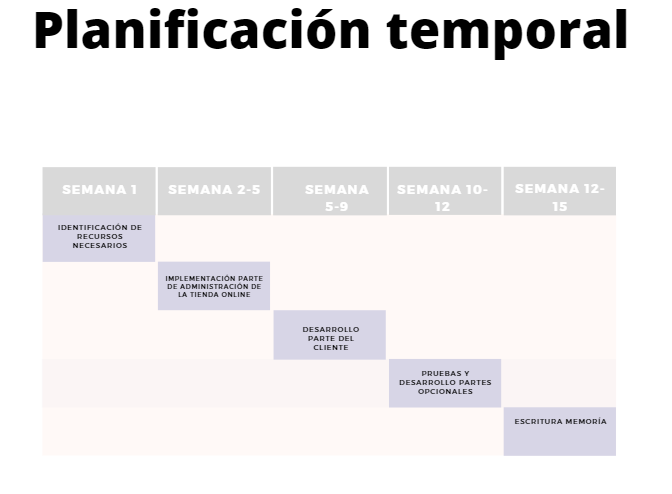
\includegraphics[width=9cm, keepaspectratio]{img/planificacion_temporal}
  \caption{Planificación temporal:Diagrama de GANTT.}
  \label{fig:GANTT}
\end{figure}


%%%%%%%%%%%%%%%%%%%%%%%%%%%%%%%%%%%%%%%%%%%%%%%%%%%%%%%%%%%%%%%%%%%%%%%%%%%%%%%%
%%%%%%%%%%%%%%%%%%%%%%%%%%%%%%%%%%%%%%%%%%%%%%%%%%%%%%%%%%%%%%%%%%%%%%%%%%%%%%%%
% ESTADO DEL ARTE %
%%%%%%%%%%%%%%%%%%%%%%%%%%%%%%%%%%%%%%%%%%%%%%%%%%%%%%%%%%%%%%%%%%%%%%%%%%%%%%%%

\cleardoublepage
\chapter{Estado del arte}
\label{chap:estado}


Para el desarrollo de este trabajo fin de grado se han utilizado diferentes tecnologías, las cuales se explicarán a continuación. 



\section{HTML5} 
\label{sec:HTML5}

HTML5 (Hyper Text Markup), es la quinta y última versión de HTML, lenguaje estándar utilizado para la definición y estructuración de los contenidos de las páginas web.

Se trata de una versión muy diferente a versiones anteriores, ya que su desarrollo vino dado por discrepancias entre diferentes miembros del consorcio W3C. En el año 2004, WATWG (Web HyperText Application Technology Working Group) sacó una primera versión, para el asombro de todos. Pero, fue en el año 2009 y, en colaboración con WATWG, cuando W3C comenzó con el desarrollo de la especificación de HTML5. 

Fue creado con la intención de sustituir a la versión anterior de HTML (HTML4). Pero, también se pretendía que la aparición de esta nueva versión relevará otros lenguajes como XHTML1 y DOM Nivel 2. 

Esta versión, además de incluir nuevas etiquetas y atributos, proporciona una plataforma de desarrollo para la creación de aplicaciones web complejas. Entre las nuevas funcionalidades se encuentran los siguientes puntos:   

\begin{itemize}
\item Incorporación de elementos multimedia para reproducir sonidos y videos desde el propio navegador. Estos elementos multimedia, son las etiquetas $<audio>$ y $<video>$.
\item Integración de gráficos vectoriales escalables (SVG).
\item Incorporación del elemento $<canvas>$, el cual permite dibujar y recrear animaciones en el navegador.
\item Almacenamiento local en el lado del cliente, con $localStorage$ y $SeassionStorage$.
\item Incorporación de etiquetas que permiten la estructuración de los documentos HTML, sin recurrir al uso de $<div>$. Entre estas etiquetas, se encuentran $<header>$ y $<footer>$, muy útiles para la creación de la cabecera y el pie de la página HTML.
\item Incorporación de $MathML$ para el manejo de fórmulas matemáticas en los documentos web.  


\end{itemize}

\section{CSS3} 
\label{sec:CSS3}

CSS3 (Cascading Style Sheets), es la última versión de CSS. Es un lenguaje de programación que permite definir y crear el aspecto visual de los documentos web. 

Surgío de la necesidad de los desarrolladores de separar el contenido de estos documentos web de su estilo, ya que, de este modo, permitía crear documentos web más simples. Además, permite que un mismo documento web tenga varias hojas de estilo, facilitando así, por ejemplo, el diseño responsive, ya que una misma información necesita estilos distintos para los diferentes tipos de pantalla. Del mismo modo, que un documento puede tener varias hojas de estilo, una misma hoja puede ser reutilizada en varios documentos web, simplificando el trabajo de los desarrolladores. 

Es un lenguaje simple, que se basa en reglas para definir los aspectos visuales del documento web. Como resumen, su propio nombre es capaz de propocionar la información necesaria que define el lenguaje, siendo esta la siguiente: 

\begin{itemize}
\item Cascading: Este término indica que el estilo que se aplica al elemento padre del documento web también se aplica a los elementos hijos que contenga, propagándose en forma de cascada. 
\item Style: Como ya se ha mencionado anteriormente, es un lenguaje que define el estilo, aspecto visual del contenido de los documentos web. 
\item Sheets: Los estilos se añaden en ficheros, hojas cuya extensión es .css. Estas hojas son utilizadas en los diferentes documentos web o en el mismo documento, permitiendo así la simplicidad y flexibilidad en los documentos web. 

\end{itemize}

Algunas de las novedades más importantes que introduce esta versión de css son: transicciones, sombras en cajas, gradientes, esquinas redondeadas, múltiples imágenes en fondo, opacidad o tranparencia de los colores, entre otras. 

Para finalizar, mencionar que el encargado de definir y mantener las especificaciones de este lenguaje es Worl Wide Web Consortium (W3C).

\section{JavaScript} 
\label{sec:JavaScript}

JavaScript es un lenguaje de programación interpretado, no necesita ser compilado para poder ejecutarse. Esto hizo que muchos usuarios de páginas web dudarán sobre la seguridad del código. Pero para eso, JavaScript se creó para funcionar en un entorno limitado, es decir, que el código JavaScript no puede acceder a los recursos del propio ordenador. A raíz de esto, los navegadores también definieron sus propias normas de seguridad, las cuáles determinan que un script no puede establecer conexión con páginas que pertenezcan a diferentes dominios. 

Además, es un lenguaje orientado a objetos y eventos. Está basado en prototipos, en vez de usar clases para la herencia utiliza prototipos que, simulan muchas de las características que tienen las clases en los lenguajes de programación orientados a objetos, como puede ser Java. 

Es un lenguaje imperativo y estructurado. Aunque su nombre puede indicar que tiene mas relación con Java, la realidad es muy distinta, pues tanto la semántica como los propósitos de ambos lenguajes son diferentes. Unas de las principales características en cuanto a este lenguaje de programación y que lo difiere de otros muchos lenguajes es el ámbito de las variables. Pues, en Javascript el ámbito de las variables es la función donde han sido declaradas y no el bloque en el cuál se declaran. Con la versión 6, se introdujo esta mejora, permitiendo que la variable fuese usada en el bloque siempre y cuando se definiese utilizando el término $let$.  
 
Es un lenguaje débilmente tipado y dinámico, es decir, una misma variable puede adoptar dos tipos de datos diferentes en distintos momentos sin tener que redefinir la variable. Está formado en su totalidad por objetos, puediéndose modificar las propiedades de dichos objetos en tiempo de ejecución, dontándolo así del dinamismo que lo define.  

Es un lenguaje rápido y ligero, por lo que se convierte en uno de los lenguajes más usuados en el mundo del desarrollo de aplicaciones web. Su uso, principalmente, está en el lado del cliente pero, con la aparición de tecnologías como NodeJS, el uso de JavaScript en el lado del servidor está sufriendo un repunte significativo. El hecho de ser un lenguaje multiplaforma, que permite utilizarse tanto en Windows, como en Linux como en Mac, así como en cualquier navegador hace que aumente su popularidad y su uso. 



Surgío de la necesidad de los desarrolladores de crear páginas web complejas y dinámicas, ya que HTML únicamente permite crear documentos web estáticos. Fue desarrollado por Brendan Eich de la compañia NetScape y, su primer nombre fue Mocha. Poco tiempo después cambiaría su nombre original y pasaría a llamarse LiveScript. En el año 1995, NetScape y Sun MicroSystems (creadores del lenguaje Java) reintroducirían el lenguaje en el mundo de la programación, como Javascript. En el año 1997 se adopta como un estándar ECMA, denominándose ECMAScript. Desde entonces ha ido evolucionando  y mejorando, creándose librerías y frameworks que facilitan la programación. En el año 2015 se publicó ECMAScript 2015 ó JavaScript 6, introduciendo características propias de las clases utilizadas en la programación orientada a objetos. La última versión hasta el momento, es la versión 8, segunda versión que tiene un proceso de desarrollo abierto. 


\section{TypeScript} 
\label{sec:TypeScript}

TypeScript es un lenguaje de programación de alto nivel orientado a objetos, de código abierto y libre. 

Su desarrollo estuvo a cargo de Microsoft y, en el, participó Anders Helsberg (diseñador y creador de C-Sharp, Delphi o Turbo Pascal). Surgió de la necesidad de los desarrollores de crear aplicaciones robustas y de gran tamaño que con el lenguaje JavaScript no podían mantener debido a su escasa escalabilidad. 

Su uso está permitido tanto en el lado del cliente, Angular 2, framework de JavaScript, usa TypeScript como lenguaje, como en el lado del servidor con NodeJS. 

TypeScript, es un "Superset" de JavaScript, es un lenguaje escrito encima de otro lenguaje. Esto significa, que TypeScript se compila a JavaScript, permitiendo que cualquier código desarrollado en JavaScript funcione sin tener que modificar el código ni la aplicación. Mejora y arregla algunos problemas que tiene el lenguaje JavaScript y, es por ello, que pone a disposición de los desarrolladores las funcionalidades disponibles en JavaScript ES6 y JavaScript ES7. Añade objetos basados en clase, facilitando la programación orientada a objetos. En su código se puede incluir ficheros de definición que contienen información de las librerías JavaScript. Además, incluye un tipado estático. El poder definir variables y funciones tipadas sin perder la esencia de JavaScript ayuda al desarrollador a evitar errores en tiempo de ejecución. Los tipos admitidos por TypeScript son: String, Number, Boolean, Array, Tuple (tipo de dato similar al Array pero con un número fijo de elementos), Enum, Any (la variable o función puede ser de cualquier tipo), Void, Never (tipo de datos que nunca se producen). 

Su publicación fue en el año 2012 y actualmente, se encuentra en la versión 2.0, la cual introduce numerosas características con respecto a la primera versión, entre las que destaca la capacidad de evitar la asiganción de varibales con un valor nulo. Aunque al principio solo existía un IDE (Microsft Visual Estudio) con TypeScript como lenguaje de programación, ahora hay numerosos editores de texto que lo incluyen como lenguaje de progración. Entre estos editores destacan Sublime Text, WebStorm, Visual Studio Code. 

Por último, destacar que su compilador también fue desarrollado en TypeScript, compilado a JavaScripy y con licencia Apache 2. 


\section{Bootstrap 4} 
\label{sec:Bootstrap 4}

BootStrap 4,  es la versión más actual y estable de Bootstrap. Bootstrap es el framework más popular de CSS. Es un conjunto de herramientas que permite a los desarrolleres mejorar el aspecto visual de los documentos HTML y de las aplicaciones web  de manera rápida y sencilla. 

Su nombre original fue Blueprint, debido a que fue creado y diseñado por Matt Otto para la compañia Twitter como herramienta de trabajo de uso interno. En el año 2011, Twitter lo libera con licencia MIT y pasa a ser de código abierto. 

El uso de este framework en las aplicaciones web permite generar diseños que, se adaptan dinámicamente a las diferentes resoluciones de pantalla y a los distintos dispositivos, favorenciendo, de este modo, el diseño conocido como responsive. Para ello, Bootstrap dispone de un sistema de cuadrilla o rejilla estándar de 940 píxeles pero, dispone de cuatro variaciones de tamaño para adaptarse a los distintos dispositivos. Estas cuatro variaciones son $sm$, $md$, $lg$ y $xl$.

Es modular y consiste en un conjunto de hojas de estilo LESS que combinado con plantillas HTML y con extensiones JavaScript implementan los diferentes componentes de Bootstrap. 

Incluye los elementos más usados en los documentos HTML, como son los formularios, las barras de progreso y de navegación, los cuadros, los mensajes de alertas o los botones con características especiales entre otros. Todos ellos tienen un estilo predefinido, pero que se puede modificar de manera sencilla. 

Para usar bootstrap en las aplicaciones web es necesario incluir en el documento HTML la hoja de estilo de Bootstrap CSS. De la misma forma, si se quiere utilizar algunos de los componentes JavaScript predefinidos de BootStrap se debe incluir la librería JQuery de JavaScript. 

La versión 4 significa una mejora en diversos componentes permitiendo un diseño más responsive. Por eso, se han modificado componentes como la navegación, que incluye la nueva clase $flexbox$. Se ha creado un nuevo componente Card que sustituye a los componente Wells, Panlles y Thumbnails. Se han modificado los elementos de paginación y las modales. Y, se incorpora el componente Grid. Además, de estas significativas mejoras, se han incluido numerosas clases de uso común. 

Por último, destacar que es compatible con todos los navegadores modernos, Firefox, Chrome, Safari, Opera, EDGE, Internet Explore 10 pero, no es compatible con las versiones anteriores a internet explorer 10.



\section{Angular} 
\label{sec:Angular}

Es un framework de código abierto diseñado por Google. Permite crear aplicaciones web de una sóla página, lo que se denomina SPA (Single Page Application). Utiliza TypeScript y HTML para el desarrollo de las aplicaciones web. 

Angular permite separar el frontend del backend y sigue un modelo MVC (Modelo-Vista-Controlador), arquitectura de software que separa los datos de la aplicación, la interfaz de usuario y la lógica de control en tres componentes distintos. Además, Angular dota a las aplicaciones de escalabilidad pues, mantiene el código ordenado. De esta forma, las modificaciones y las actualizaciones de las aplicaciones son rápidas y sencillas. 

Una de las principales ventajas de este framework y de las páginas SPA es la velocidad de carga entre las diferentes vistas de la aplicación. Cuando se cambia de vista, es decir la url se modifica, no se recarga la página sino que éstas se cargan de manera dinámica, rápida y reactiva. 

La arquitectura de una aplicación Angular se basa en clases de 4 tipos distintos (módulos, componentes, servicios y directivas). Estas clases se identifican a través de decoradores, los cuales permiten cargar los metadatos necesarios que determinan a Angular como debe usar dichas clases. 

\textbf{Módulos}.

Los módulos suministran el contexto de compilación de los componentes, es decir, es aquí donde se definen los diferentes componentes que va a formar la aplicación, las dependencias, las clases que actúan como servicios en la aplicación y las rutas de navegación que establecen las vistas de la aplicación. 

Toda aplicación angular tiene un módulo principal, que es el raíz. Este módulo suele recibir el nombre de AppModule y, es el que inicia el sistema de arranque de la aplicación. 

Al igual que en Javascript, los módulos de Angular permiten importar y exportar funcionalidades proporcionadas por otros módulos, por lo que, una aplicación puede tener más de un módulo y, cada uno de ellos ser independiente. La manera en que se organizan estos módulos ayuda a la realización de aplicaciones más complejas y a la realización de código. Además, pemite que la carga inicial sea mínima, ya que cada módulo se carga a petición, es decir, cuando se va a utilizar. 

\textbf{Componentes}. 

Las aplicaciones Angular tienen un componente que es nexo de unión entre los diferentes componentes, que forman la aplicación, y el módelo de objeto del documento de la página (DOM). Los componentes son los que tienen la lógica y los datos de la aplicación. Son los que controlan las diferentes plantillas HTML que se cargan cuando se modifican las URLs dentro de la aplicación. Estas plantillas HTML son las vistas que forman la interfaz de usuario.

De la misma forma que las aplicaciones diseñas con Angular pueden tener más de un módulo, estas aplicaciones pueden tener subcomponentes, los cuales se pueden relacionar entre sí mediante dos tipos de vinculación de datos. Mediante eventos y mediante propiedades. A través de los eventos la aplicación responde a las entradas del usuario actualizando los datos y, a través de las propiedades se envían valores calculados de los datos de la aplicación a los HTMLs que forman las vistas. Esta vinculación de datos se puede producir en ambas direcciones por lo que, igual que los datos de la aplicación pueden modificar los HTMLs, los cambios en el DOM pueden modificar los datos de la aplicación. 

Por último, decir que los componentes llevan el decorador @Component, que es el que determina a Angular que una clase actúa como un componente. 

\textbf{Servicios}

Los servicios no son más que clases en las que se definen datos o funcionalidades generales que no están asociadas a una determinada vista. Son usadas para compartir datos y operaciones entre componentes. También es donde se suele realizar toda la operativa de las peticiones a la API de las aplicaciones. Deben llevar el decorador @Injectable, pues es el que permite obtener los metados necesarios para que otras clases puedan inyectar sus dependencias. 

\textbf{Directivas}

Las directivas son clases en las que se definen los términos claves que se usan en las plantillas. Cuando se carga una vista, Angular procesa estos términos clave que modifican el HTML y el DOM de la aplicación. Por lo que, una plantilla además de utilizar HTML para definir la vista usa marcas propias de angular que son estas directivas. 

Existen dos clases de directivas, las de atributo que modifican el comportamiento del componente y, las estructurales que únicamente modifican la apariencia. 

Por último destacar la manera que tiene Angular de realizar la navegación entre las distintas vistas de la aplicación. Para ello, Angular dispone de un enrutador que no es más que un módulo que a través de un servicio define las rutas de navegación de la aplicación. Este módulo se ajusta a las convenciones de los navegadores. Esto quiere decir que, tanto si se pone la URL en la barra de direcciones como si se pincha un enlace en la aplicación como si se hace clic en el botón de retroceso o avance se navegá a la página correspondiente. El enrutador es el que muestra u oculta una vista. Cada vez que se modifica la URL el enrutador se encarga de añadir la ruta en el historial del navegador, de ahí que los botones de retroceso y avance funcionen. Cada ruta de navegación está asociado a un componente. 

Como todos los framework Angular dispone de varias versiones aportando todas ellas mejoras en dicho framework. La primera versión de Angular se conoce como AngularJS y es la más distinta a las demás pues el resto son actualizaciones de Angular 2. Cuando se definió la segunda versión se decidió modificar el nombre del framework y dejarlo como Angular. La última versión estable es la versión 8.

\subsection{Angular CLI} 
\label{sec:Angular CLI}

Angular CLI (Command Line Interface) es una herramienta de línea de comandos creada por el equipo de Angular. Es muy útil a la hora de iniciar una aplicación web diseñada con Angular, ya que con un sólo comando genera el esqueleto de carpetas y archivos necesarios de la aplicación. Además, contiene herramientas predefinidas que ayudan al desarrollo y mantenimiento de este tipo de aplicaciones. Al crear una aplicación web con Angular Cli, dentro de la estructura de archivos, se crea un archivo de configuración, en el cúal se añaden las dependencias necesarias para que la aplicación web compile y ejecute. Este archivo de configuración se va modificando conforme se van creando los componentes, servicios o directivas. Para ello, Angular Cli tiene comandos que permiten crear estas clases de manera sencilla, pues se crean los distintos archivos que conforman un componente, un servicio o una directiva. Entre las herramientas predefinidas destaca el compilador, el sistema de testing y el servidor web. 

\subsection{Angular Material} 
\label{sec:Angular Material}

Angular Material es una librería creada por Google para las aplicaciones web desarrolladas con Angular. Al igual que Boostrap ayuda a diseñar aplicaciones web atractivas, con estilos y formas únicas, ya que contiene multitud de componentes con estilos prefijados. Estos componentes permiten a las aplicaciones web ser rápidas, consistentes y versátiles. Además, con el uso de esta librería las aplicaciones web se adaptan mejor a la mayoría de resoluciones de pantalla y de dispositvos, facilitando el diseño responsive de las aplicaciones. También, con su uso se crean aplicaciones web accesibles, ya que los componentes cumplen con los estándares de accesibilidad. Mencionar que al utilizar esta librería se facilita la internacionalización de la aplicación puesto que, permite la utilización de diferentes idiomas. Por último, destacar que es compatible con todos los navegadores modernos. 

\subsection{Angular Editor} 
\label{sec:Angular Editor}

Es un componente de angular que permite escribir texto con formato y estilo propio dentro de un documento HTML. El estilo y el formato lo determina el usuario, por lo tanto el estilo como el formato puede variar de un usuario a otra y de un texto a otro. El componente transforma lo escrito con el formato y el estilo definido al lenguaje HTML para que en pantalla se visualice conforme el usuario determina. Es compatible únicamente con las últimas versiones de angular, siendo estas Angular 6, Angular 7 y Angular 8. 

\subsection{Node.js} 
\label{sec:Node.js}
Node js fue creado en 2009 por Ryan Dahl como sistema de desarrollo de aplicaciones red escalables. Es un entorno de ejecución orientado a eventos asíncronos que utiliza el motor V8 de Google, desarrollado en C++ y de código abierto, para interpretar el código javascript, del mismo modo que hace el navegador Chrome. 

Se basa en sistemas como Event Machine de Ruby y Twisted de Python, con la diferencia que Node.js no necesita realizar la llamada de bloqueo de inicio de evento que tienen estos sistemas, si no que cuando ejecuta el script de entrada del bucle inicio de eventos arranca y finaliza cuando no hay más devoluciones de llamadas callbacks, utilizando así un único hilo por conexión. De este modo, cada nuevo evento se añade al bucle de eventos que se ejecuta al inicio, evitando el bloqueo de procesos que se produce en los sistemas de concurrencias basados en la utilización de hilos de los sistemas operativos. Estos procesos usan un hilo por cada conexión provocando la ineficiencia de los recursos utilizados. A pesar de que Node.js esté pensado para usar un único hilo se pueden crear hilos diferentes o subprocesos a través de Apis propias de Node como API_child.process.fork(). 

Por otro lado Node es un buen aliado para desarrollar aplicaciones web, ya que a la hora de implementar el protocolo Http para Node se pensó tanto en la latencia de transmisión como en la transimisión por streaming de datos. 

\section{Npm} 
\label{sec:Npm}
Npm es el sistema de administración de paquetes del entorno de ejecución JavaScript NodeJs. Dicho sistema contiene un cliente, a través del cual ejecutando una línea de comando se instalan los paquetes necesarios para que un proyecto NodeJs funcione correctamente y, una biblioteca o base de datos con más de 477000 paquetes disponibles para poder usarse. Todos estos paquetes están guardados con formato CommonsJs y contienen un archivo para almacenar metadatos con formato Json. Fue desarrollado por Isaac Z. Schlueter y se desarrollo por completo en JavaScript.

Al instalar un paquete a través de Npm, se instala baja el directorio del proyecto \slash .node\_modules. Permite instalar con un único comando todas las dependencias del proyecto NodeJs, siempre y cuando se ejecute el comando en la raíz del proyecto. Esto es debido a que Npm utiliza el archivo con formato Json, denominado Package.json para guardar todos los metadatos relevantes a los modulos, paquetes y dependencias del proyecto. Por ejemplo, en el archivo package.json se pueden guardar las versiones válidas para los diferentes módulos, así como hacer un versionado del modulo instalado para que a la hora de auto actualizarse no se estropee el proyecto. Gracias a esto, Npm hace que la instalación de proyectos NodeJs, descargados de Git sea sencilla.

\section{Express.js} 
\label{sec:Express.js}


\section{Git} 
\label{sec:Git}

Git es un software de control de versiones. Fue diseñado por Linus Torvalds. Es un software libre que se distribuye a través de la versión 2.0 de GNU. 

Git permite el trabajo en equipo, ya que fomenta el desarrollo no lineal de los proyectos. Esto es debido al sistema de ramas que tiene. En cada rama se puede trabajar sobre una funcionalidad distinta, agilizando de esta forma el desarrollo del proyecto y, haciendo que el trabajo en equipo sea más sencillo y óptimo. Además, permite gestionar de manera eficiente aplicaciones y proyectos de grandes envergaduras. 

Los cambios en los proyectos se realizan de manera inmediata, ya que cada desarrollador tiene una copia en local (en su equipo) del proyecto. Esto permite navegar por el historial de cambios sin necesidad de conectarse a un servidor. Es decir, se puede trabajar en local hasta finalizar una tarea y, posteriormente subirlo a la nube. Así, todo el equipo obtiene el cambio en su proyecto local. 

Permite tener una copia del proyecto en la nube, por lo que a la hora de desarrollar grandes proyectos te proporciona tranquilidad, ya que puedes obtener una copia o versión anterior aún habiéndose roto el equipo.

Cuando se usa Git en un equipo de trabajo se definen flujos que determinan como se va a realizar el desarrollo del proyecto. Lo habitual, es que exista una rama master, la cual será la que siempre se depliegue en producción. De esta rama master se obtiene una nueva rama, denominada develop. Esta rama develop es la que va a tener todos los cambios y todas las funcionalidades del proyecto y, es la que se va a mezclar con la rama master. Para funcionalidades específicas se crean ramas que se obtienen de la develop y que se suelen llamar features. De esta forma, se permite el desarrollo en paralelo de los distintos integrantes del grupo. Una vez que la funcionalidad esté finalizada y probada se junta con la rama develop. Al actualizar los demás miembros del equipo su rama develop, se obtienen los cambios de las nuevas funcionalidades sin que se vea afectado el trabajo que cada uno está realizando. Cuando en producción hay un error y debe ser solucionado inmediatamente, se crea una rama a partir de la master y, es sobre esta rama donde se desarrollan las soluciones al error. Esta rama se mezcla con la rama master de nuevo y se denomina hotfix. Cuando los errores son menores y, no son urgentes no hace falta crear ramas hotfix, si no que se crean ramas, llamadas issues, en las que que se solucionan todos los posibles errores de una versión. Una vez solucionados los errores, la rama se mezcla con la rama master y con la develop.

\section{Visual Studio Code} 
\label{sec:Visual Studio Code}

Visual Studio Code es un editor de código fuente, lanzado en noviembre de 2015 por Microsoft. Desde entonces, ha sufrido numerosas actualizaciones hasta llegar a la última versión 1.47. 

Puede ser instalado en los sistemas operativos más conocidos: Linux, Windows y Macos. 

Soporta una gran cantidad de lenguajes de programación. El resaltado de sintaxis, la capacidad de finalización del código que se escribe, la refactorización del código, el modo depuración así como la integración con Git facilita el desarrollo de aplicaciones. 

Para hacer más atractiva su interfaz y para facilitar su uso, permite personalizar los temas del editor y los atajos del teclado. 

Es un editor de código abierto, lo que quiere decir que se puede descargar de GitHub y realizar cualquier modificación en su código. Se basa en Electron, framework utilizado para el desarrollo de aplicaciones de escritorio usando tecnologías web, utiliza Chromium para el motor gráfico y NodeJs para ejecutar JavaScript.
%%%%%%%%%%%%%%%%%%%%%%%%%%%%%%%%%%%%%%%%%%%%%%%%%%%%%%%%%%%%%%%%%%%%%%%%%%%%%%%%
%%%%%%%%%%%%%%%%%%%%%%%%%%%%%%%%%%%%%%%%%%%%%%%%%%%%%%%%%%%%%%%%%%%%%%%%%%%%%%%%
% DISEÑO E IMPLEMENTACIÓN %
%%%%%%%%%%%%%%%%%%%%%%%%%%%%%%%%%%%%%%%%%%%%%%%%%%%%%%%%%%%%%%%%%%%%%%%%%%%%%%%%

\cleardoublepage
\chapter{Diseño e implementación}

Aquí viene todo lo que has hecho tú (tecnológicamente). 
Puedes entrar hasta el detalle. 
Es la parte más importante de la memoria, porque describe lo que has hecho tú.
Eso sí, normalmente aconsejo no poner código, sino diagramas.

\section{Arquitectura general} 
\label{sec:arquitectura}

Si tu proyecto es un software, siempre es bueno poner la arquitectura (que es cómo se estructura tu programa a ``vista de pájaro'').

Por ejemplo, puedes verlo en la figura~\ref{fig:arquitectura}.
\LaTeX \ pone las figuras donde mejor cuadran. 
Y eso quiere decir que quizás no lo haga donde lo hemos puesto...
Eso no es malo.
A veces queda un poco raro, pero es la filosofía de \LaTeX: tú al contenido, que yo me encargo de la maquetación.

\begin{figure}
  \centering
  \includegraphics[width=9cm, keepaspectratio]{img/arquitectura}
  \caption{Estructura del parser básico.}
  \label{fig:arquitectura}
\end{figure}

Recuerda que toda figura que añadas a tu memoria debe ser explicada.
Sí, aunque te parezca evidente lo que se ve en la figura~\ref{fig:arquitectura}, la figura en sí solamente es un apoyo a tu texto.
Así que explica lo que se ve en la figura, haciendo referencia a la misma tal y como ves aquí.
Por ejemplo: En la figura~\ref{fig:arquitectura} se puede ver que la estructura del \emph{parser} básico, que consta de seis componentes diferentes: los datos se obtienen de la red, y según el tipo de dato, se pasará a un \emph{parser} específico y bla, bla, bla\ldots

Si utilizas una base de datos, no te olvides de incluir también un diagrama de entidad-relación.


%%%%%%%%%%%%%%%%%%%%%%%%%%%%%%%%%%%%%%%%%%%%%%%%%%%%%%%%%%%%%%%%%%%%%%%%%%%%%%%%
%%%%%%%%%%%%%%%%%%%%%%%%%%%%%%%%%%%%%%%%%%%%%%%%%%%%%%%%%%%%%%%%%%%%%%%%%%%%%%%%
% RESULTADOS %
%%%%%%%%%%%%%%%%%%%%%%%%%%%%%%%%%%%%%%%%%%%%%%%%%%%%%%%%%%%%%%%%%%%%%%%%%%%%%%%%

\cleardoublepage
\chapter{Resultados}

En este capítulo se incluyen los resultados de tu trabajo fin de grado.

Si es una herramienta de análisis lo que has realizado, aquí puedes poner ejemplos de haberla utilizado para que se vea su utilidad.


%%%%%%%%%%%%%%%%%%%%%%%%%%%%%%%%%%%%%%%%%%%%%%%%%%%%%%%%%%%%%%%%%%%%%%%%%%%%%%%%
%%%%%%%%%%%%%%%%%%%%%%%%%%%%%%%%%%%%%%%%%%%%%%%%%%%%%%%%%%%%%%%%%%%%%%%%%%%%%%%%
% CONCLUSIONES %
%%%%%%%%%%%%%%%%%%%%%%%%%%%%%%%%%%%%%%%%%%%%%%%%%%%%%%%%%%%%%%%%%%%%%%%%%%%%%%%%

\cleardoublepage
\chapter{Conclusiones}
\label{chap:conclusiones}


\section{Consecución de objetivos}
\label{sec:consecucion-objetivos}

Esta sección es la sección espejo de las dos primeras del capítulo de objetivos, donde se planteaba el objetivo general y se elaboraban los específicos.

Es aquí donde hay que debatir qué se ha conseguido y qué no. 
Cuando algo no se ha conseguido, se ha de justificar, en términos de qué problemas se han encontrado y qué medidas se han tomado para mitigar esos problemas.

Y si has llegado hasta aquí, siempre es bueno pasarle el corrector ortográfico, que las erratas quedan fatal en la memoria final.
Para eso, en Linux tenemos aspell, que se ejecuta de la siguiente manera desde la línea de \emph{shell}:

\begin{verbatim}
  aspell --lang=es_ES -c memoria.tex
\end{verbatim}

\section{Aplicación de lo aprendido}
\label{sec:aplicacion}

Aquí viene lo que has aprendido durante el Grado/Máster y que has aplicado en el TFG/TFM. Una buena idea es poner las asignaturas más relacionadas y comentar en un párrafo los conocimientos y habilidades puestos en práctica.

\begin{enumerate}
  \item a
  \item b
\end{enumerate}


\section{Lecciones aprendidas}
\label{sec:lecciones_aprendidas}

Aquí viene lo que has aprendido en el Trabajo Fin de Grado/Máster.

\begin{enumerate}
  \item Aquí viene uno.
  \item Aquí viene oto.
\end{enumerate}


\section{Trabajos futuros}
\label{sec:trabajos_futuros}

Ningún proyecto ni software se termina, así que aquí vienen ideas y funcionalidades que estaría bien tener implementadas en el futuro.

Es un apartado que sirve para dar ideas de cara a futuros TFGs/TFMs.


%%%%%%%%%%%%%%%%%%%%%%%%%%%%%%%%%%%%%%%%%%%%%%%%%%%%%%%%%%%%%%%%%%%%%%%%%%%%%%%%
%%%%%%%%%%%%%%%%%%%%%%%%%%%%%%%%%%%%%%%%%%%%%%%%%%%%%%%%%%%%%%%%%%%%%%%%%%%%%%%%
% APÉNDICE(S) %
%%%%%%%%%%%%%%%%%%%%%%%%%%%%%%%%%%%%%%%%%%%%%%%%%%%%%%%%%%%%%%%%%%%%%%%%%%%%%%%%

\cleardoublepage
\appendix
\chapter{Manual de usuario}
\label{app:manual}

Esto es un apéndice.
Si has creado una aplicación, siempre viene bien tener un manual de usuario.
Pues ponlo aquí.

%%%%%%%%%%%%%%%%%%%%%%%%%%%%%%%%%%%%%%%%%%%%%%%%%%%%%%%%%%%%%%%%%%%%%%%%%%%%%%%%
%%%%%%%%%%%%%%%%%%%%%%%%%%%%%%%%%%%%%%%%%%%%%%%%%%%%%%%%%%%%%%%%%%%%%%%%%%%%%%%%
% BIBLIOGRAFIA %
%%%%%%%%%%%%%%%%%%%%%%%%%%%%%%%%%%%%%%%%%%%%%%%%%%%%%%%%%%%%%%%%%%%%%%%%%%%%%%%%

\cleardoublepage

% Las siguientes dos instrucciones es todo lo que necesitas
% para incluir las citas en la memoria
\bibliographystyle{abbrv}
\bibliography{memoria}  % memoria.bib es el nombre del fichero que contiene
% las referencias bibliográficas. Abre ese fichero y mira el formato que tiene,
% que se conoce como BibTeX. Hay muchos sitios que exportan referencias en
% formato BibTeX. Prueba a buscar en http://scholar.google.com por referencias
% y verás que lo puedes hacer de manera sencilla.
% Más información: 
% http://texblog.org/2014/04/22/using-google-scholar-to-download-bibtex-citations/

\end{document}
